\documentclass[a4paper, tikz]{article}

%--------------------use package--------------------%
\usepackage{xeCJK}
\usepackage[left=2.5cm,right=2cm,top=2cm,bottom=2cm]{geometry}
\setmainfont{TimesNewRomanPSMT}%设置英文字体
\setCJKmainfont{STSongti-SC-Regular}%设置中文字体
\usepackage{indentfirst} 
\usepackage{hyperref}
\usepackage{natbib}
\usepackage{titlesec}
\usepackage{titletoc}
\usepackage{setspace}%行间距
\usepackage{enumitem} 
\usepackage{booktabs}
\usepackage[justification=centering]{caption}
\usepackage{subcaption}
\usepackage{float}
\usepackage{color}
\usepackage{amsfonts}
\usepackage{array}
\usepackage{tikz}
\usepackage{pgfplots}
\usetikzlibrary{positioning}
\usepackage{amsmath}
\usepackage{setspace}

%--------------------fontset--------------------%

\setCJKfamilyfont{song}{STSongti-SC-Regular}
\newcommand{\song}{\CJKfamily{song}} 
\setCJKfamilyfont{hei}{STHeitiSC-Light}
\newcommand{\hei}{\CJKfamily{hei}}
\setCJKfamilyfont{kai}{STKaitiSC-Regular} 
\newcommand{\kai}{\CJKfamily{kai}} 

\newcommand{\chuhao}{\fontsize{42pt}{\baselineskip}\selectfont}     %初号
\newcommand{\xiaochuhao}{\fontsize{36pt}{\baselineskip}\selectfont} %小初号
\newcommand{\yihao}{\fontsize{28pt}{\baselineskip}\selectfont}      %一号
\newcommand{\erhao}{\fontsize{21pt}{\baselineskip}\selectfont}      %二号
\newcommand{\xiaoerhao}{\fontsize{18pt}{\baselineskip}\selectfont}  %小二号
\newcommand{\sanhao}{\fontsize{15.75pt}{\baselineskip}\selectfont}  %三号
\newcommand{\sihao}{\fontsize{14pt}{\baselineskip}\selectfont}%     四号
\newcommand{\xiaosihao}{\fontsize{12pt}{\baselineskip}\selectfont}  %小四号
\newcommand{\wuhao}{\fontsize{10.5pt}{\baselineskip}\selectfont}    %五号
\newcommand{\xiaowuhao}{\fontsize{9pt}{\baselineskip}\selectfont}   %小五号
\newcommand{\liuhao}{\fontsize{7.875pt}{\baselineskip}\selectfont}  %六号
\newcommand{\qihao}{\fontsize{5.25pt}{\baselineskip}\selectfont}    %七号

%%------------------------------标题名称中文化-----------------------------%
\renewcommand{\contentsname}{\hei 目录}
%\renewcommand {\listfigurename }{图目录}
%\renewcommand {\listtablename }{表目录}
%\renewcommand {\partname }{第\thepart 部}
%\renewcommand {\chaptername }{第\thechapter 章}
%\renewcommand{\figurename}{图\thesection\ -}
\renewcommand{\figurename}{图}
%\renewcommand{\thefigure}{\oldstylenums{\thesection}-\oldstylenums{\arabic{figure}}}
\renewcommand{\tablename}{表}
%\renewcommand{\thetable}{\oldstylenums{\thesection}-\oldstylenums{\arabic{table}}}
%\renewcommand {\bibname }{参考文献}
%\renewcommand {\appendixname }{附录}
%\renewcommand {\indexname }{索引}
\renewcommand{\abstractname}{}
\renewcommand{\refname}{\hei 参考文献}

%%------------------------------定理名称中文化-----------------------------%
%\newtheorem{dingyi}{\hei 定义~}[section]
%\newtheorem{dingli}{\hei 定理~}[section]
%\newtheorem{yinli}[dingli]{\hei 引理~}
%\newtheorem{tuilun}[dingli]{\hei 推论~}
%\newtheorem{mingti}[dingli]{\hei 命题~}
%\newtheorem{lizi}{{例}}

\titleformat{\section}{\bfseries\sihao\hei}{\thesection .\quad}{0pt}{}
\titleformat{\subsection}{\bfseries\xiaosihao\hei}{\thesubsection \quad}{0pt}{}
\titleformat{\subsubsection}{\bfseries\wuhao\hei}{\thesubsubsection \quad}{0pt}{}
\titleformat{\paragraph}{\wuhao\song}{}{}{}{}

%\definecolor{orange}{RGB}{255,140,0}
%\definecolor{bleu}{RGB}{0,140,255}

%\renewcommand{\thetable}{\thechapter{}.\arabic{table}}
%\renewcommand{\thefigure}{\thechapter{}.\arabic{figure}}


\makeatletter\@addtoreset{equation}{section}
\makeatother\renewcommand\theequation{\oldstylenums{\thesection}-\oldstylenums{\arabic{equation}}}

%--------------------title--------------------%
\title{\bfseries\xiaoerhao\hei 基于级联卷积和递归神经网络的蛋白质二级结构预测}
\author{\bfseries\xiaosihao\kai 电子与信息工程学院\qquad 计算机科学与技术\\
\xiaosihao\kai 118532014013\qquad 袁\ 超\qquad 指导教师:游文杰}
\date{}

%--------------------main document--------------------%
\begin{document}
\setcitestyle{super}%设置文献引用模式为右上角

% 题目
\maketitle

\setlength{\parindent}{2em}

% 摘要
{\bfseries\xiaowuhao\kai 
\subparagraph{\hei【摘\quad 要】}蛋白质二级结构预测(PSSP)是生物信息学中的一个重要问题。受深度学习在自然语言处理领域成功启发,本文提出了一种端到端的深度神经网络模型,用于预测八类蛋白质二级结构。模型主要包含四个层次:首先,基于氨基酸残基的类别信息、生物的进化信息以及蛋白质序列的组成信息进行编码组合,利用特征嵌入来消除0-1矩阵的稀疏性;其次,使用多尺度卷积提取氨基酸残基之间的局部相邻特征;然后,通过门控单元(GRU)双向递归神经网络提取蛋白质序列的远程上下文关系;最后,融合局部相邻特征以及远程上下文关系来进行八类蛋白质二级结构预测。实验结果表明,本文提出的深度神经网络模型易于收敛,具有较好的可扩展性。预测效果良好,在CB513数据集上达到了68.2\%的$Q_8$预测精度。

\subparagraph{\hei【关键词】}蛋白质二级结构预测;深度神经网络
}
\newpage

% 目录 
\tableofcontents
\newpage

% 正文
\section{引言}
\subsection{背景及现状}%介绍该问题领域背景:什么人做过什么事儿,主要技术有哪些
\subsubsection{背景知识}
蛋白质是生命的物质基础,也是细胞中不可缺少的分子成份。各种不同形式的生命活动都与蛋白质发生着紧密的联系,如:催化化学反应的酶、控制体内信号的受体以及人体的肌肉和器官组织\citep{liu2016overview} 等。随着蛋白质研究的不断进行,先进的测序技术也随之发展,蛋白质组学应用而生。人们可以利用成熟的技术手段\citep{hunt1986protein}测量蛋白质的序列,或是从已有的开放数据库中查询具有相似组成的蛋白质。迄今为止,已有大量测序蛋白质不断被填入到数据库中,呈现出了指数级上升的趋势\citep{jiang2017protein}。

与测序不同,测量蛋白质的结构困难重重。对于已知序列的蛋白质,可以被确定具体结构的微乎其微\citep{li2011novel}。传统实验方法,例如X射线晶体学和核磁共振光谱\citep{ho2012survey},精度高但耗时长,而且造价昂贵,不能够应对蛋白质序列快速增长的挑战。通过采用先进的计算机技术,高效地处理大量蛋白质序列数据,降低了经济成本和时间负担。因此,采用计算方法进行蛋白质结构预测成为了交叉学科生物信息学领域重要而有趣的课题。

蛋白质结构可划分为四个等级:一级为氨基酸序列,决定了蛋白质的折叠方式;二级描述了多肽的局部现象;三级为全局折叠模式;四级反应了蛋白质高度紧凑和相互作用的结果。蛋白质三级结构和四级结构是高度立体的三维状态,决定了蛋白质的功能特征。在一级结构到三级结构之间,二级结构起到了承接和桥梁的作用。因此,蛋白质二级结构预测(Protein Secondary Structure Prediction,PSSP)是蛋白质结构预测中必不可少的步骤。

\subsubsection{发展现状}
PSSP最早追溯到20世纪80年代,利用统计模型估算不同二级结构中特定氨基酸出现的概率\citep{levitt1976structural} 。考虑到该方法特征不充分,识别率较低,所以结合多种特征信息(亲/疏水性等理化性质),以及复杂统计方法(多肽等局部相关作用)进行了改进,但总体改善效果甚微\citep{zhang2005improving} 。20世纪90年代,位置特异得分矩阵(Position-specific Scoring Matrices,PSSM)通过提取蛋白质家族的进化信息\citep{jones1999protein} ,预测效果实现了显著提升。21世纪,优秀的机器学习算法层出不穷,在共同考虑进化信息的前提之下结合不同机器学习算法,如:人工神经网络、支持向量机以及概率图模型等\citep{wu1995neural}\citep{gewehr2005ssep}\citep{asai1993prediction} 。近些年,集成多种模型的组合方法,可以克服单个模型固有的缺陷所带来的性能问题。不同种模型间互补,这是一种新的趋势\citep{bidargaddi2009combining}。然而,现有模型多为非序列模型,这些模型不是蛋白质二级结构的理想模型,这是因为蛋白质序列不能以固定维数作为载体。此外,几乎所有方法都是基于3类PSSP,当涉及更具挑战的八类PSSP问题时,进展停滞不前。

近年来,得益于更强大的计算机、更庞大的数据集和训练更深网络的技术,一种通用的表征学习的方法:深度学习(Deep Learning)流行起来。传统技术的表示方法完全由手工设计,而深度学习中更复杂的表示是由简单表示组合而成,并使用通用的学习过程从数据中学习而来。事实证明,深度学习非常擅长发现高维数据中错综复杂的结构关系\citep{lecun2015deep} 。

\subsection{本文主要工作}
本文从蛋白质问题的概述展开,介绍了相关的课题背景以及发展现状。对八类蛋白质二级结构预测的问题做了更精确的描述,并从探讨预测问题出发,介绍了机器学习相关背景知识,包括机器学习最核心的训练模式:监督学习,以及采用经验风险最小化策略和梯度下降算法来进行模型优化。然后,具体介绍了深度神经网络中的一些最基础、最重要的计算模型,并利用这些模型组建深度神经网络来做预测。接着,进行实验,测试该模型的具体效果。最后,做分析和总结。


\subsection{论文组织结构}
本课题共分为六章,章节内容安排如下:

\begin{description}[itemindent=2em]
	\item[第一章(引言)] 介绍课题的相关背景和发展现状,主要工作,以及论文的结构和安排。
	\item[第二章(蛋白质预测概述)] 介绍了蛋白质基础知识,八类二级结构预测的具体问题,监督学习以及优化策略等,还有常用的预测评估标准。
	\item[第三章(深度学习简介)] 介绍了感知机模型,卷积神经网络模型以及GRU递归神经网络模型。
	\item[第四章(模型架构)] 介绍了本文提出深度神经网络模型,包括:编码、组合嵌入层、多尺度卷积层、双向GRU层以及预测层。
	\item[第五章(实验分析)] 介绍了数据集以及具体实验过程。
	\item[第六章(总结)] 总结本文的工作成果。
\end{description}
\newpage

\section{蛋白质预测概述}
\subsection{符号表}
表1中列举了在本文中使用的符号及其意义

\begin{table}[p]
\renewcommand\arraystretch{1.2}
\caption{主要符号表}
\center
\begin{tabular}{p{120pt}<{\centering} p{280pt}<{\centering}}
\toprule
常用符号& 意义\\
\midrule
$x$ & 蛋白质序列\\
$y$ & 二级结构\\
$X$ & 蛋白质输入样本\\
$Y$ & 二级结构预测结果\\
$f$ & 二级结构预测模型\\
$f_{\theta}$ & 带训练参数$\theta$的预测模型\\
$\hat{f}$ & 估计模型\\
$x^{(i)}$ & 蛋白质序列第$i$个残基\\
$y^{(i)}$ & 二级结构中第$i$个位置所对应类别\\
$x_i$ & 样本中第$i$条蛋白质\\
$y_i$ & 第$i$条蛋白质的二级结构\\
$\theta$ & 参数向量\\
$\eta$ & 学习率\\
$\sigma$ & 激活函数\\
$*$ & 卷积运算\\
$I$ & 矩阵\\
$h^{(t)}$ & 动态系统在$t$时刻的状态\\
$e^{(t)}$ & 表示序列在$t$位置的fofe编码\\
$A$ & 编码层的输出\\
$B$ & B-GRUs层的输出\\
$C$ & 多尺度卷积层的输出\\
$J$ & 模型复杂度\\
$\nabla_{\theta} J$ & 模型复杂度对参数$\theta$的梯度值\\
$concatenate\{\}$ & 对应残基间进行拼接组合\\
$\{A,C,D,\cdots\}_{20}$ & 20种氨基酸\\
$\{H,G,I,\cdots\}_{8}$ & 八类二级结构\\
$\mathbb{X}={\{A,C,D,\cdots\}_{20}}^n$ & 输入空间,表示所有可能的蛋白质输入\\
$\mathbb{Y}={\{H,G,I,\cdots\}_{8}}^n$ & 预测空间,表示所有可能的二级结构预测\\
$w=(w_1,w_2,\cdots,w_n)^T$ & 权值向量\\
$W_z,W_r,W_h,U_z,U_r,U_h$ & GRU训练参数\\
\bottomrule
\end{tabular}
\end{table}

\subsection{二级结构预测}%预测问题的符号化定义
\subsubsection{组成及结构}
蛋白质作为重要的生物大分子,其化学化学组成及比例:碳(50\%)、氢(7\%)、氧(23\%)、氮(16\%)、硫(0.3\%)其他元素微量。所有蛋白质都来自20种不同的L型$\alpha$氨基酸(A、C、D、E、F、G、H、I、K、L、M、N、P、Q、R、S、T、V、W和Y),氨基酸有氨基($\rm -NH_2$)和羧基($\rm -COOH$),两两间可以脱去一分子水($\rm H_2O$)缩合形成肽键($\rm -CO-NH-$)进而组成多肽,此时的氨基酸也被称作残基。通常认为,残基数目达到一定规模,便可称其为蛋白质的一级结构。

蛋白质结构可以分为四个层次,层与层之间可以转化,每一层的结构都与上一层的结构关系密切。图1为蛋白质PDB\ 105M的四层结构示意图。观察该蛋白质的二级结构和三级结构,可以发现在三级结构中存在有许多螺旋,这些螺旋都可以从二级结构中找到一一对应的位置,螺旋的数目和长度也完全被定义。并且,在二级结构中,这些螺旋都沿着蛋白质一级结构的序列方向,循环折叠而成。每个残基都有一个二级结构类别标签,连续相邻的残基具有相同的标签,则在空间中体现为一段蛋白质序列的空间折叠。这说明二级结构可以初步呈现出蛋白质的局部空间状态,想要从大量已知的蛋白质序列预测复杂多变的空间结构,可以将二级结构预测作为首要环节。

\begin{figure}[htbp]
\begin{subfigure}{0.5\textwidth}
	\centering
	\begin{subfigure}{1\textwidth}
		{\qihao%105M的各级结构
  		\quad\\
  		VLS\textcolor[RGB]{255,0,0}{EGEWQLV\quad LHVWAKVEA}\textcolor[RGB]{0,155,0}{D}\quad \textcolor[RGB]{255,0,0}{VAGHGQDILI\quad RLFKS}H\textcolor[RGB]{255,0,0}{PETL}\quad \textcolor[RGB]{0,155,0}{EK}F\textcolor[RGB]{0,155,0}{DRFKH}LK\quad \textcolor[RGB]{0,155,0}{T}\textcolor[RGB]{255,0,0}{EAEMKA}S\textcolor[RGB]{255,0,0}{ED\quad LKKHGVTVLT\quad ALGAIL}\textcolor[RGB]{0,155,0}{KKKG}\quad HH\textcolor[RGB]{255,0,0}{EAELKPLA\quad QSHAT}\textcolor[RGB]{0,155,0}{KH}KIP\quad \textcolor[RGB]{255,0,0}{IKYLEFISEA\quad IIHVLHSR}\textcolor[RGB]{0,155,0}{HP\quad GDF}G\textcolor[RGB]{255,0,0}{ADAQGA\quad MNKALELFRK\quad DIAAKYKEL}\textcolor[RGB]{0,155,0}{G}\quad YQG\quad}
  		\caption{}
	\end{subfigure}
	\newline\newline\newline
	\begin{subfigure}{1\textwidth}
  		\centering
  		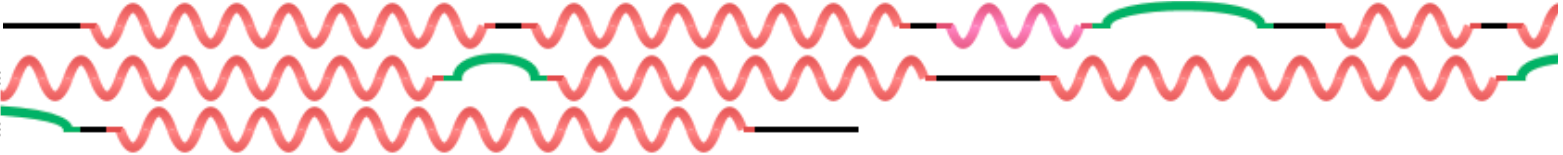
\includegraphics[width=\linewidth, trim=7 4 7 4,clip]{pic/105M_ss.png}
  		\caption{}
	\end{subfigure}
\end{subfigure}
\begin{subfigure}{.25\textwidth}
  \centering
  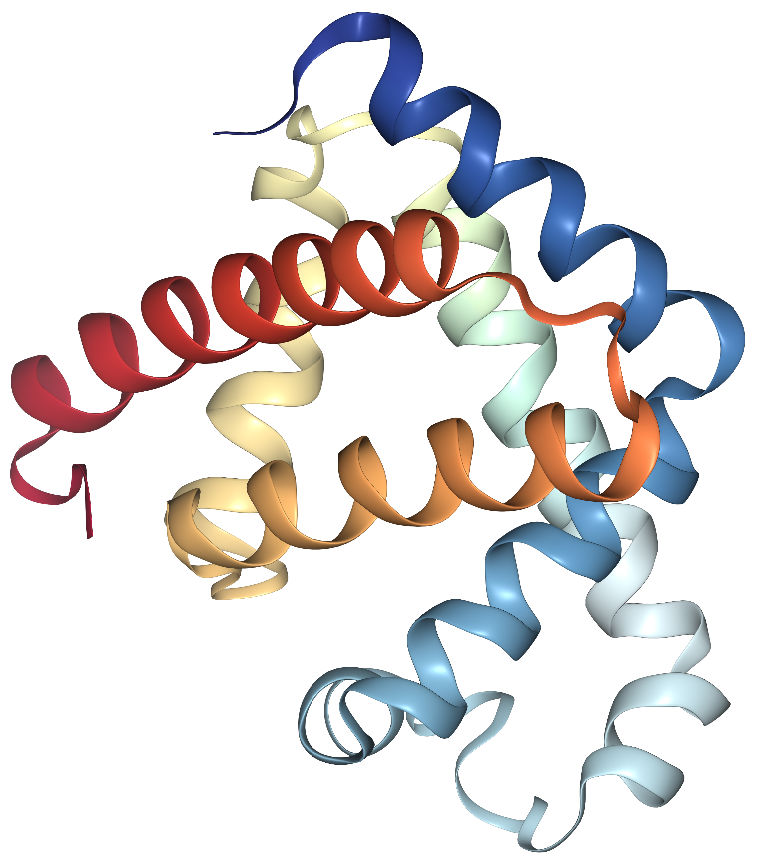
\includegraphics[height=.8\linewidth]{pic/105M_ts.jpg}
  \caption{}
\end{subfigure}%
\begin{subfigure}{.25\textwidth}
  \centering
  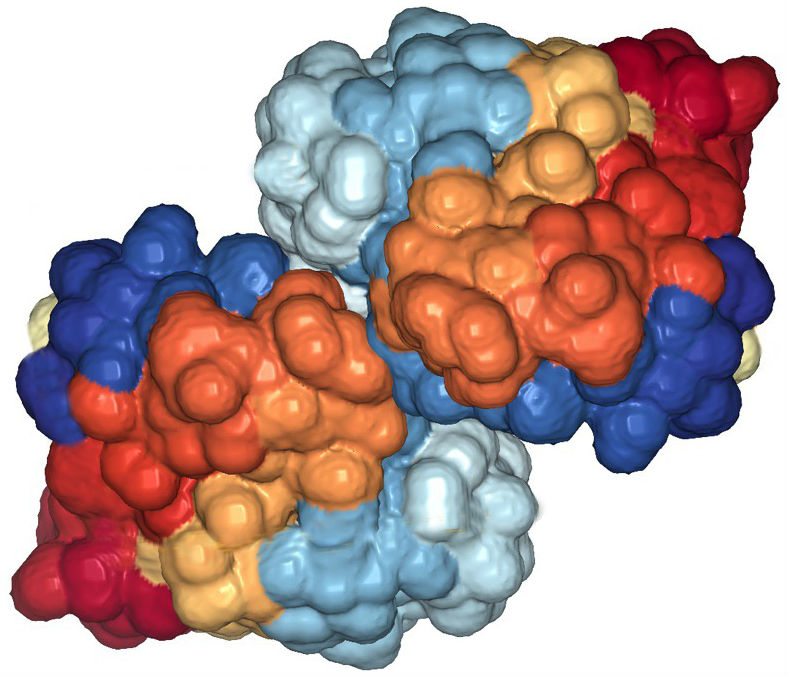
\includegraphics[height=.8\linewidth]{pic/105M_fs.jpg}
  \caption{}
\end{subfigure}
\caption{
数据来自RCSB(\url{https://www.rcsb.org/})的蛋白质PDB\ 105M:a)为该蛋白质氨基酸序列,字母代表不同种类的氨基酸残基;b)为该蛋白质的3类二级结构图,颜色代表的类别与(a)中的色彩相对应;c)代表其三级结构的彩虹带图;d)为两条105M蛋白质相互结合形成的四级结构表面图。}
\label{fig:fig}
\end{figure}

在早期的研究中,蛋白质的二级结构被划分为三类:螺旋、折叠和转角。之后分类方式不断丰富。根据二级结构定义词典\citep{bulut2007dssp} 可将残基分为八个类别:H($\alpha-$螺旋)、G($310-$螺旋)、I($\pi-$螺旋)、E($\beta-$折片)、B($\beta-$桥)、T(转角)、S(卷曲)以及C(其他)。基于八类的PSSP方法可以提供更详细的局部结构信息,也更具挑战性。本课题主要研究八类二级结构预测问题,所以之后提到的PSSP均指八类二级结构预测。

\subsubsection{八类预测}
给定一组蛋白质输入序列$X=\{x_1,x_2,\cdots,x_N\}$,存在$f:X\to Y$即,对于每个$x_i\in X$,$y_i\in Y$,都有
\begin{equation}
	y_i=f(x_i)
\end{equation}
则称$f$为蛋白质二级结构的预测模型,$Y$为输入集$X$的预测结果,$N$为样本容量。特别的,令$x=(x^{(1)},x^{(2)},\cdots,x^{(n)})^T$,$x\in X$,$x^{(i)}\in \{A,C,D,\cdots\}_{20}$为第$i$个残基,$n$是该序列的长度。若存在模型$f$,使得
\begin{equation}
	y=f(x)=(y^{(1)},y^{(2)},\cdots,y^{(n)})^T
\end{equation}
如果$y^{(i)}\in \{H,G,I,E,B,T,S,C\}_8$,则称$y$为序列$x$的八类二级结构预测结果,$y^{(i)}$为第$i$个残基所对应的二级结构,共八种类别。

我们已经形式化的定义了什么是PSSP,即我们要学习什么样的模型,解决什么问题。下一小节将介绍一种最常见的学习形式——监督学习,以及如何用梯度下降实现该学习。

\subsection{学习、策略以及评估}
\subsubsection{监督学习}
首先,给定一组蛋白质二级结构训练样本
\begin{equation}
	T=\{(x_1,y_1),(x_1,y_1),\cdots,(x_N,y_N)\}
\end{equation}
其中$(x_i,y_i)$,$i=1,2,\cdots,N$,称作训练样本点,
\begin{align}
	x_i=(x_i^{(1)},x_i^{(2)},\cdots,x_i^{(n)})^T\\
	y_i=(y_i^{(1)},y_i^{(2)},\cdots,y_i^{(n)})^T
\end{align}
$x_i\in X\subseteq \mathbb{X}$,$x_i$为输入的观测值,$\mathbb{X}={\{A,C,D,\cdots\}_{20}}^n$为蛋白质序列的输入空间,$y_i\in Y\subseteq \mathbb{Y}$为输出观测值,$\mathbb{Y}={\{H,G,I,\cdots\}_8}^{n}$,为预测空间。假设训练数据与测试数据依联合概率分布$P(X,Y)$独立同分布产生,在未给出测试数据的情况下,监督学习模型可以从训练数据得到
\begin{equation}
	\hat{f}	= arg\ max\{P|\hat{P}(Y|X)\}
\end{equation}
$\hat{P}(Y|X)$表示由训练样本观测到的条件概率分布,是从数据中学到的经验,也可称模型$f$\citep{周志华2016机器学习}。因为训练集有多组,所以我们学到的经验不唯一。我们从这组经验中选择“最优”($arg\ max$)的分布$P$,既为我们通过训练样本所估计的模型$\hat{f}$。更普遍的,机器学习模型通常包含一个参数向量$\theta$
\begin{equation}
	{\hat{f}}_{\theta}=arg\ max\{P|\hat{P_{\theta}}(Y|X),\theta\in {\mathbb{R}}^n\}
\end{equation}
参数向量$\theta$的维度由具体模型决定,并会在学习过程中不断被修正,直至模型收敛到最优。

\subsubsection{梯度下降}
PSSP问题为典型的多类别分类问题,所以设估计模型$\hat{f_{\theta}}$的损失函数为
\begin{equation}	
	L(y_j, \hat{f}_{\theta}(x_j))=-\sum_{i=1}^{n}y_j^{(i)}\log \hat{f}_{\theta}(x_j)^{(i)}
\end{equation}
则其代价函数:
\begin{equation}
	J_{\theta}=\frac{1}{N}\sum_{j=1}^{N}L(y_j, \hat{f}_{\theta}(x_j))	
\end{equation}
$J_{\theta}$反应了模型在观测样本中的拟合效果,当观测样本$N$趋近于无穷,我们可以学习到最理想的模型,代价函数也可以达到最低值0。所以,我们说优化模型,就是训练参数$\theta$使得$J_{\theta}$趋于0。我们也把这种策略称为经验风险最小化(Empirical Risk Minimization,ERM)策略\citep{李航2012统计学习方法} 。

若$\hat{f_{\theta}}$为线性模型,最小化代价函数可以转化成凸优化问题,即求$\partial J_{\theta}$的零界点。但PSSP问题是高维非线性复杂性问题,也称NP(Non-deterministic, Polynomial)问题\citep{lathrop1994protein} ,无法在多项式时间内被确定地求解,所以我们只关注一些较小值或是局部极小值,并利用迭代、梯度下降来优化该解,具体的:
\begin{equation}
	\theta \gets \theta - \eta \frac{\partial J_{\theta}}{\partial \theta}
\end{equation}
其中$\eta$为学习率。通常,在深度学习中模型非常复杂,难以求出${\partial J_{\theta}}/{\partial \theta}$的具体解析式,我们常用梯度$\nabla_{\theta} J$来替代,并利用反向传播(Backpropagation,BP)的方法来近似地计算。将$\eta$设置为一个较小的值,每次进行小步的迭代。迭代过程中$\theta$总会沿着梯度下降的方向进行更新,即$J_{\theta}$越来越接近于最小值,从而到达局部极小值点。

\subsubsection{预测评估}
为了客观评价预测的性能,需要选取一些评估指标。PSSP问题最常用的评估指标是$Q_8$准确率,设第$i$条蛋白质序列$x_i$有$n_i$个残基,其中正确预测有$m_i$个残基,则
\begin{equation}
	Q_8=\frac{\sum\limits^{N}_{i=1}m_i}{\sum\limits^{N}_{i=1}n_i}
\end{equation}
第$i$条蛋白质的$Q_8$准确率
\begin{equation}
	q_i = \frac{m_i}{n_i}
\end{equation}
也可以参考准确率
\begin{equation}
	r=\frac{1}{N}\sum\limits^{N}_{i=1}\frac{m_i}{n_i}
\end{equation}

\subsection{本章小结}
本章介绍了蛋白质二级结构预测的基础知识。下一章主要介绍一些计算模型方法。

\newpage


\section{深度学习简介}%这一块还要延伸,一些技术细节,公式推导
首先回顾一些基本概念。

\subsection{神经元与深度}
神经元(Neuron)是神经网络中最基础的成分,各种复杂的网络结构都是由一个个小的神经元连接构成。其中,最简单的设计是感知机(Perceptron),一种包含有多个输入的感知机模型如图3所示。

\begin{figure}[htbp]
\centering
\begin{tikzpicture}
\tikzset{basic/.style={draw,fill=black!30!white,rounded corners, text width=1.6em, text badly centered,thick}}
\tikzset{input/.style={basic,circle}}
\tikzset{weights/.style={basic,rectangle}}
\tikzset{functions/.style={basic,circle,fill=black!30!white,draw,align=center, inner sep=1pt,
  font=\sffamily}}
	\fill[gray!20, rounded corners] (0.4,-2.35) -- (0.4,1.4) -- (-3.4,1.4) -- (-3.4,-2.35) -- cycle;
	\node[functions] (center) {};
	\draw[thick,draw] (0.5em,0.5em) -- (0,0.5em) -- (0,-0.5em) -- (-0.5em,-0.5em);
	\draw (0em,0.75em) -- (0em,-0.75em);
	\draw (0.75em,0em) -- (-0.75em,0em);
	\node[right of=center, font=\scriptsize](right){输出};
		\path[draw,->,thick] (center) -- (right);
	\node[functions,draw,left=2em of center,dashed] (left) {$\sum$};
		\path[draw,thick] (left) -- (center);	
	\node[left=2.5em of left](dots){$\vdots$} -- (dots) node[left of=dots](ldots){$\vdots$};
	\node[weights,draw,above of=dots,fill=black!15] (1) {$w^{(1)}$} -- (1) node[weights,draw,left of=1,fill=black!15] (l1) {$x^{(1)}$};
		\path[draw,->,thick] (l1) -- (1);
		\path[draw,->,thick] (1) -- (left);
	\node[weights,draw,below of=dots,fill=black!15] (n) {$w^{(n)}$} -- (n) node[weights,draw,left of=n,fill=black!15] (ln) {$x^{(n)}$};
		\path[draw,->,thick] (ln) -- (n);
		\path[draw,->,thick] (n) -- (left);		
	\node[weights,draw,below of=n,fill=black!15](b){$b$};
		\path[draw,->,thick] (b) -- (left);	
	\node[below of=b,font=\scriptsize] (w){连接权重};
	\node[below of=ln,font=\scriptsize] {输入};
	\node[below of=center,font=\scriptsize,text width=3em] {激活函数};
\end{tikzpicture}
\caption{多输入感知机模型}
\label{fig:fig}
\end{figure}

\begin{equation}
	f_{\theta}= \sigma(\sum_{i=1}^{n}w^{(i)}x^{(i)}+b)
\end{equation}
特别的,$\theta=(w^{(1)},w^{(2)},\cdots,w^{(n)},b)^T$。$\sigma$为激活函数,常见的激活函数有:S函数$Sigmoid$、双曲正切函数$tanh$,线性整流函数$ReLU$以及归一化指数函数$Softmax$\citep{glorot2010understanding} 。

\begin{align}
	sigmoid(x)&=\frac{1}{1+e^{-x}}\\
	tanh(x)&=\frac{e^x-e^{-x}}{e^x+e^{-x}}\\
	ReLU(x)&=\begin{cases}
	0.01x,\quad x\l 0 \\
	x,\quad x\ge 0
	\end{cases}\\
	Softmax(x)^{(j)}&=\frac{e^{x^{(j)}}}{\sum_{n}^{i=1}e^{x^{(i)}} }
\end{align}

感知机只在输出时进行一次激活,所以学习能力非常有限。事实上,感知机可以灵活组合,使用多个感知机学习可以得到多个输出,多分类神经网络模型中经常可以见到类似的结构。并且也可以将感知机的输出作为新的输入,这就是我们常说的多层神经网络,对应的总层数即是所谓的模型的深度(Depth)。

这种由一层的输出作为下一层的输入的结构是非常灵活的,我们可以用其他计算结构替换对应的子结构。下一小节将会介绍两种常用的计算结构:卷积神经网络(Convolutional Neural Network, CNN)和递归神经网络(Recursive Neural Networks),这是深度学习中最重要的,也是最基础技术\citep{liu2017protein}\citep{guo2018protein} 。

\subsection{卷积神经网络}
卷积神经网络是一种专门处理矩阵的神经网络,卷积神经网络中每层都由若干卷积单元组成,其中的参数称为核函数,记为$K$。
\begin{equation}
	K = \{w_1,w_2,\cdots,w_k\}
\end{equation}
设卷积核$w\in K$,$w$与矩阵$I$进行一次卷积运算,则矩阵$I$第$i$行第$j$列的运算结果为:
\begin{equation}
	I'_{i,j}= (I*w)_{i,j}=\sum_{m}\sum_{n}I_{i+m,j+n}w_{m,n}
\end{equation}
$(m\times n)$为卷积核$w$的尺寸,$*$为卷积运算,$I'$为单个卷积的输出,上标$'$表示输出$I'$的尺寸与输入不同,发生了改变。若$K$中卷机核数目为$k$,则单层卷机的输出为$A$:
\begin{equation}
	A = ReLU((I*K)+b)
\end{equation}
\begin{equation}
	A = \{I'_1,I'_2,\cdots,I'_k\}
\end{equation}

\subsection{递归神经网络}%\subsection{其他相关知识}%正则化:L2正则化提前终止、
与卷积神经网络的核函数不同,循环神经网络的子结构是一个动态系统
\begin{equation}
	h^{(t)} = f_{\theta}(h^{(t-1)},x^{(t)})
\end{equation}
$h^{(t)}$称为系统在$t$时刻的状态也可称为$t$时刻的输出,$x^{(t)}$是$t$时刻给定的输入。系统在$t$时刻展开形式
\begin{equation}
	h^{(t)} = g_{\theta}^{(t)}(x^{(t)},x^{(t-1)},\cdots,x^{(1)},h^{(1)},h^{(2)},\cdots,h^{(t-1)})
\end{equation}
若保存所有迭代的输出,循环神经网络模型可以构建出如下的映射关系:
\begin{equation}
	f_{\theta}:\{x^{(1)},x^{(2)},\cdots,x^{(t)}\}\to \{h^{(1)},h^{(2)},\cdots,h^{(t)}\}
\end{equation}
注意,这里映射两边都是集合的形式,表示该模型也和神经网络模型一样非常灵活。我们可以只保留第$t$时刻的输出状态$h^{(t)}$,模型为$n\to1$;也可以保留第$i$到第$t$时刻输出$\{h^{(i)},\cdots,h^{(t)}\}$,模型变成了$n\to m$;也可以令$x^{(t+1)}\gets h^{(t)}$,模型又变成了$m\to n$或$1\to n$,其中$n$和$m$满足$n>m>1$。

因为循环神经网络会考虑$t$时刻的状态,所以结构具备学习“因果”的能力\citep{mikolov2010recurrent} 。但蛋白质二级结构和序列的关系是整体依赖的,我们不能说蛋白质第$i$位置的二级结构只和从第$1$到第$i-1$的序列相关而与第$i+1$后面的序列无关。双向循环神经网络\citep{petridis2018end} 则是为满足该需求而设计的,具体思路是沿着时间$t$的反方向再输入一次,训练一层新的网络,这样输出集比原来扩大了一倍,包含了更丰富的输出结果。

普通的循环神经网络无法处理随模型不断递归导致的权重爆炸或梯度消失的问题(Vanishing gradient problem)。近几年提出的具备“遗忘功能”的模块:长短时间记忆(Long-Short Term Memory ,LSTM)和门控循环单元(Gated Recurrent Unit,GRU)被广泛用于训练循环网络\citep{chung2014empirical}\citep{gers1999learning} ,具有类似模块的可以递归训练的神经网络又被称为递归神经网络(Recursive Neural Networks,RNN)。LSTM和GRU在实验中表现效果相当\citep{goodfellow2016deep} ,但GRU的参数更少,约为LSTM的$3/4$,所以训练速度更快。GRU的结构如图$3$。

\begin{align}
z^{(t)} &= \sigma(W_z x^{(t)}\oplus  U_z h^{(t-1)}+b_z)\\
r^{(t)} &= \sigma(W_r x^{(t)}\oplus U_r h^{(t-1)}+b_r)\\
h'^{(t)}&= tanh(W_h x^{(t)}\oplus U_h(r^{(t)}\otimes h^{(t-1)})+b_h)\\
h^{(t)} &= z^{(t)}\otimes h^{(t-1)}+(1-z^{(t)})\otimes h'^{(t)}
\end{align}

$z^{(t)}$是控制更新的门控,$r^{(t)}$是控制重置的门控,$h'^{(t)}$包含了当前输入$x^{(t)}$以及历史信息$h^{(t-1)}$。当$z^{(t)}=0$时,当前状态$h^{(t)}$和历史状态$h^{(t-1)}$之间为非线性函数。若同时有$z=0$,$r=1$时,GRU单元退化为简单的循环网络;若同时有$z=0$,$r=0$,当前状态$h^{(t)}$只和当前输入$x^{(t)}$相关,和历史状态$h^{(t-1)}$无关。当$z=1$时,当前状态等于上一时刻的状态$h^{(t-1)}$,和当前输入$x^{(t)}$无关。

\newpage
\begin{figure}[htbp]
\centering
\begin{tikzpicture}
\tikzset{basic/.style={draw,rounded corners,thick,text badly centered}}
\tikzset{yuan/.style={basic, circle, text width=1.5em, thick, align=center, inner sep=1pt,
  font=\sffamily,
  fill=black!30}}
\tikzset{fang/.style={basic, rectangle, text width=2.3em, very thick,
  fill=black!15}}
\tikzset{jian/.style={basic, draw, thick,->}}
\tikzset{xian/.style={basic, draw, thick}}

\fill[gray!20, rounded corners] (1.3,1.2) -- (9.3,1.2) -- (9.3,7.5) -- (1.3,7.5) -- cycle;

\node[fang](21)at(2,0.5){$x^{(t)}$};
\node[fang](07)at(0.5,7){$h^{(t-1)}$};
\node[fang](24)at(2,4){$z^{(t)}$};
\node[fang](44)at(4,4){$r^{(t)}$};
\node[fang](94)at(8.5,4){$h'^{(t)}$};
\node[fang](97)at(8.5,7){$h^{(t)}$};

\node[yuan,dashed](22)at(2,2){$\bigoplus$};
\node[yuan](23)at(2,3){$\sigma$};
\node[yuan,dashed](27)at(2,7){$\bigotimes$};
\node[yuan](42)at(4,2){$\sigma$};
\node[yuan,dashed](45)at(4,5){$\bigotimes$};
\node[yuan,dashed](46)at(3,6){$1-$};
\node[yuan,dashed](64)at(6,4){$\bigoplus$};
\node[yuan,dashed](66)at(6,6){$\bigotimes$};
\node[yuan,dashed](67)at(6,7){$+$};
\node[yuan](74)at(7,4){$tanh$};


\node[yuan,dashed](117)at(10.5,6.5){$\bigoplus$};
\node[right of=117, text badly centered]{\quad 向量拼接};
\node[yuan,dashed, below of=117](116){$\bigotimes$};
\node[right of=116, text badly centered]{\quad\quad\quad 向量元素相乘};
\node[yuan,dashed, below of=116](115){$+$};
\node[right of=115, text badly centered]{向量和};

\path[jian] (21) -- (22);
\path[xian] (2,1.5) -- (6,1.5) -- (64) [jian];
\path[xian] (22) -- (23);
\path[xian] (22) -- (42);
\path[jian] (23) -- (24);
\path[jian] (42) -- (44);
\path[jian] (44) -- (45);
\path[xian] (45) -- (6,5) -- (64) [jian];
\path[jian] (64) -- (74);
\path[jian] (74) -- (94);
\path[xian] (07) -- (0.5,2) -- (22) [jian];
\path[xian] (07) -- (0.5,5) -- (45) [jian];
\path[xian] (07) -- (27) [jian];
\path[xian, dashed] (24) -- (27) [jian];
\path[xian, dashed] (2,6) -- (46) [jian];
\path[jian] (27) -- (67);
\path[jian] (46) -- (66);
\path[jian] (66) -- (67);
\path[xian] (94) -- (8.5,6) -- (66)[jian];
\path[jian] (67) -- (97);
\path[jian] (97) -- (8.5,7.8);
\path[jian] (97) -- (9.7,7);
\end{tikzpicture}
\caption{GRU的结构图}
\label{fig:fig}
\end{figure}

\subsection{本章小结}
本章介绍了深度学习模型的基础知识,下一章将利用这些知识构建预测蛋白质二级结构的深度神经网络模型。
\newpage

\section{模型架构}
为解决PSSP问题,本文设计了一个深度神经网络模型架构,如图4所示。该模型主要包含:组合嵌入层、多尺度卷积层、B-GRUs层以及预测层四个层次。下面将依次详细介绍各层。

\begin{figure}[htbp]
\centering
\begin{tikzpicture}
\tikzset{nn/.style={draw, circle, fill=black}}

\tikzset{gru/.style={draw, rectangle, thick, fill=gray!20}}

\node[](seq)at(0,0){$\underbrace{VLS\cdots AKYKELGYQG\_\_\_\_\_\_\_\_\_\_\_\_\_}_{700}$};
\draw[] (-3.3,1) rectangle ++(6.6,2.4);

\draw[step=0.2] (-3.3,1) grid (3.3,1+0.6);
\fill[black] (-3.2,1+0.2) rectangle ++(.2,.2);
\fill[black] (-3,1) rectangle ++(.2,.2);
\fill[black] (-2.8,1+0.2+0.2) rectangle ++(.2,.2);
\fill[black] (-2.6,1+0.2+0.2) rectangle ++(.2,.2);
\fill[black] (-2.4,1) rectangle ++(.2,.2);
\fill[black] (-2.2,1+0.2) rectangle ++(.2,.2);
\fill[black] (-2,1) rectangle ++(.2,.2);

\fill[black] (-1.8,1) rectangle ++(.2,.2);
\fill[black] (-1.6,1+0.2+0.2) rectangle ++(.2,.2);
\fill[black] (-1.4,1+0.2) rectangle ++(.2,.2);
\fill[black] (-1.2,1+0.2+0.2) rectangle ++(.2,.2);
\fill[black] (-1,1) rectangle ++(.2,.2);

\fill[black] (-0.8,1+0.2) rectangle ++(.2,.2);
\fill[black] (-0.6,1+0.2+0.2) rectangle ++(.2,.2);
\fill[black] (-0.4,1) rectangle ++(.2,.2);
\fill[black] (-0.2,1) rectangle ++(.2,.2);
\fill[black] (-0,1+0.2) rectangle ++(.2,.2);

\fill[black] (3,1+0.2+0.2) rectangle ++(.2,.2);
\fill[black] (2.8,1+0.2) rectangle ++(.2,.2);
\fill[black] (2.6,1) rectangle ++(.2,.2);
\fill[black] (2.4,1+0.2+0.2) rectangle ++(.2,.2);
\fill[black] (2.2,1) rectangle ++(.2,.2);
\fill[black] (2,1+0.2) rectangle ++(.2,.2);

\fill[black] (1.8,1+0.2) rectangle ++(.2,.2);
\fill[black] (1.6,1+0.2) rectangle ++(.2,.2);
\fill[black] (1.4,1+0.2+0.2) rectangle ++(.2,.2);
\fill[black] (1.2,1) rectangle ++(.2,.2);
\fill[black] (1,1+0.2) rectangle ++(.2,.2);

\fill[black] (0.8,1+0.2) rectangle ++(.2,.2);
\fill[black] (0.6,1+0.2) rectangle ++(.2,.2);
\fill[black] (0.4,1+0.2+0.2) rectangle ++(.2,.2);
\fill[black] (0.2,1) rectangle ++(.2,.2);

\draw[] (-3.3,1) rectangle ++(6.6,0.6);
\node[](onehot)at(-4.2,0.8){one-hot};
\draw [->,thick] (-3.4,0.2) to [out=180, in=-90] (onehot) to [out=90, in=180] (-3.4,1.3);

\shadedraw[inner color=black, outer color=gray] (-3.3,1+0.6) rectangle ++(6.6,0.6);
\node[](pssm)at(-6,0.8){PSSM};
\draw [->,thick] (-3.4,0.1) to [out=180, in=-90] (pssm) to [out=90, in=180] (-3.4,1.9);

\shade[left color=white, right color=black] (-3.3,1+0.6+0.6) rectangle ++(6.6,0.6);
\shade[left color=black, right color=white] (-3.3,1+0.6+0.6+0.6) rectangle ++(6.6,0.6);
\draw[dashed] (-3.3,1+0.6+0.6+0.6) -- (3.3,1+0.6+0.6+0.6);
\node[](bifofe)at(5,1.9){bi-fofe};
\draw [->,thick] (3.4,1.2) to [out=0, in=-90] (bifofe) to [out=90,in=0] (3.4,2.8);


\draw[dashed, red,  thick] (-3,0.9) rectangle ++(0.2,2.6);
\draw[->,thick, red] (-3.1,3.5) to [out=180, in=-90] (-4.3,4) to [out=90, in=160] (-3.1,4.3);

\node[nn](11)at(-2,4.2){};
\node[nn](12)at(0,4.2){};
\node[nn](13)at(2,4.2){};

\node[nn](21)at(-3,5){};
\node[nn](22)at(-1,5){};
\node[nn](23)at(1,5){};
\node[nn](24)at(3,5){};

\draw[thick] (11) -- (21);
\draw[thick] (11) -- (22);
\draw[thick] (11) -- (23);
\draw[thick] (11) -- (24);

\draw[thick] (12) -- (21);
\draw[thick] (12) -- (22);
\draw[thick] (12) -- (23);
\draw[thick] (12) -- (24);

\draw[thick] (13) -- (21);
\draw[thick] (13) -- (22);
\draw[thick] (13) -- (23);
\draw[thick] (13) -- (24);

\draw[] (6,6) rectangle ++(2,3);
\draw[dashed, red,  thick](5.9,6.2) rectangle ++(2.2,.2);
\draw[->,thick, red] (3.3,5) to [out=0, in=-120] (9,5.3) to [out=60, in=0] (8.2,6.3);

\draw[dashed, blue,  thick](5.9,7.4) rectangle ++(2.2,1.2);


\draw[dashed] (4,8) rectangle ++(1.4,3);
\filldraw[opacity=0.3,color=gray] (4+0.2,8+0.2) rectangle ++(0.3,2.0);
\filldraw[opacity=0.3,color=gray] (4+0.2+0.1,8+0.2+0.1) rectangle ++(0.3,2.0);
\filldraw[opacity=0.3,color=gray] (4+0.2+0.2,8+0.2+0.2) rectangle ++(0.3,2.0);
\node[xslant=1](d)at(4+1,8+1.8){$\vdots$};
\filldraw[opacity=0.3,color=gray] (4+0.2+0.2+0.2+0.2+0.1,8+0.2+0.2+0.2+0.2+0.1) rectangle ++(0.3,2.0);
\draw[->,thick, blue] (5.8,8.6) to (5.5,9);

\draw[dashed] (2,7) rectangle ++(1.4,3);
\filldraw[opacity=0.3,color=gray] (2+0.2,7+0.2) rectangle ++(0.3,2.0);
\filldraw[opacity=0.3,color=gray] (2+0.2+0.1,7+0.2+0.1) rectangle ++(0.3,2.0);
\filldraw[opacity=0.3,color=gray] (2+0.2+0.2,7+0.2+0.2) rectangle ++(0.3,2.0);
\node[xslant=1](d)at(2+1,7+1.8){$\vdots$};
\filldraw[opacity=0.3,color=gray] (2+0.2+0.2+0.2+0.2+0.1,7+0.2+0.2+0.2+0.2+0.1) rectangle ++(0.3,2.0);
\draw[->,thick, blue] (5.8,8) to (3.5,8.6);

\draw[dashed] (3.6,4.8) rectangle ++(1.4,3);
\filldraw[opacity=0.3,color=gray] (3.6+0.2,4.8+0.2) rectangle ++(0.3,2.0);
\filldraw[opacity=0.3,color=gray] (3.6+0.2+0.1,4.8+0.2+0.1) rectangle ++(0.3,2.0);
\filldraw[opacity=0.3,color=gray] (3.6+0.2+0.2,4.8+0.2+0.2) rectangle ++(0.3,2.0);
\node[xslant=1](d)at(3.6+1,4.8+1.8){$\vdots$};
\filldraw[opacity=0.3,color=gray] (3.6+0.2+0.2+0.2+0.2+0.1,4.8+0.2+0.2+0.2+0.2+0.1) rectangle ++(0.3,2.0);
\draw[->,thick, blue] (5.8,7.4) to (5.1,6.4);


\draw[] (-5,7.5) rectangle ++(1.4+1.4+1.4,3);
\draw[] (-5,7.5) rectangle ++(1.4,3);
\draw[->,thick,dashed] (4-0.2,8+3-0.2-0.5) to [out=-120,in=-30] (-5+1.4+1.4+0.7,7.5+3-2);

\draw[] (-5+1.4,7.5) rectangle ++(1.4,3);
\draw[->,thick,dashed] (2-0.2,7+3-0.2-0.5-1.6) to [out=-180,in=-30] (-5+1.4+0.7,7.5+3-2);

\draw[] (-5+1.4+1.4,7.5) rectangle ++(1.4,3);
\draw[->,thick,dashed] (3.6-0.2,4.8+3-0.2-0.5-1.3) to [out=-230,in=-30] (-5+0.7,7.5+3-2);

\draw[ thick,dashed, red] (-5-0.1,7.5+2.6) rectangle ++(1.4+1.4+1.4+0.2,0.2);

\draw[->,thick,red] (-5-0.1,7.5+2.6) to [out=120,in=-90] (-7.5,15-0.3);


\draw[dashed] (-7,12) rectangle ++(3.4,3);
\node[gru]() at (-7+0.7,12+2.6){GRU};
\node[]() at (-7+0.7+1,12+0.7){$\vdots$};
\node[gru]() at (-7+0.7+2,12+1.5){GRU};
\draw[->, thick] (-7+0.7-1.2,12+2.6+0.1) to (-7+0.7-0.5,12+2.6+0.1);
\draw[->, thick] (-7+0.7-1.2+1.7,12+2.6+0.1) to (-7+0.7-0.5+3+0.7,12+2.6+0.1);
\draw[->, thick] (-7+0.7-1.2,12+2.6+0.1) to (-7+0.7-0.5+2,12+1.5+0.1);
\draw[->, thick] (-7+0.7,12+2.6+0.1-0.35) to (-7+0.7,12+2.6+0.1-1);
\draw[->, thick] (-7+0.7+2,12+1.5+0.1+0.15) to (-7+0.7+2,12+1.5+0.1+0.75);
\draw[->, thick] (-7+0.7-0.5+3,12+1.4+0.1) to (-7+0.7-0.5+3+0.7,12+2.6);


\draw[] (-3,12) rectangle ++(1.4,3);
\draw[dashed,thick,red] (-3-0.1,12+2.6) rectangle ++(1.4+0.2,0.2);

\draw[dashed] (-1,12) rectangle ++(3.4,3);
\node[gru]() at (-1+0.7,12+2.6){GRU};
\node[]() at (-1+0.7+1,12+0.7){$\vdots$};
\node[gru]() at (-1+0.7+2,12+1.5){GRU};
\draw[->, thick] (-1+0.7-1.2,12+2.6+0.1) to (-1+0.7-0.5,12+2.6+0.1);
\draw[->, thick] (-1+0.7-1.2+1.7,12+2.6+0.1) to (-1+0.7-0.5+3+0.7,12+2.6+0.1);
\draw[->, thick] (-1+0.7-1.2,12+2.6+0.1) to (-1+0.7-0.5+2,12+1.5+0.1);
\draw[->, thick] (-1+0.7,12+2.6+0.1-0.35) to (-1+0.7,12+2.6+0.1-1);
\draw[->, thick] (-1+0.7+2,12+1.5+0.1+0.15) to (-1+0.7+2,12+1.5+0.1+0.75);
\draw[->, thick] (-1+0.7-0.5+3,12+1.4+0.1) to (-1+0.7-0.5+3+0.7,12+2.6);


\draw[] (3,12) rectangle ++(1.4,3);
\draw[dashed,thick,red] (3-0.1,12+2.6) rectangle ++(1.4+0.2,0.2);

\draw[dashed] (5,12) rectangle ++(3.4,3);
\node[gru]() at (5+0.7,12+2.6){GRU};
\node[]() at (5+0.7+1,12+0.7){$\vdots$};
\node[gru]() at (5+0.7+2,12+1.5){GRU};
\draw[->, thick] (5+0.7-1.2,12+2.6+0.1) to (5+0.7-0.5,12+2.6+0.1);
\draw[->, thick] (5+0.7-1.2+1.7,12+2.6+0.1) to (5+0.7-0.5+3+0.7,12+2.6+0.1);
\draw[->, thick] (5+0.7-1.2,12+2.6+0.1) to (5+0.7-0.5+2,12+1.5+0.1);
\draw[->, thick] (5+0.7,12+2.6+0.1-0.35) to (5+0.7,12+2.6+0.1-1);
\draw[->, thick] (5+0.7+2,12+1.5+0.1+0.15) to (5+0.7+2,12+1.5+0.1+0.75);
\draw[->, thick] (5+0.7-0.5+3,12+1.4+0.1) to (5+0.7-0.5+3+0.7,12+2.6);

\draw[] (9,12) rectangle ++(1.4,3);
\draw[dashed,thick,red] (9-0.1,12+2.6) rectangle ++(1.4+0.2,0.2);


\draw[] (-1.4-1.4-1.4,16) rectangle ++(1.4+1.4+1.4+1.4+1.4+1.4,3);
\draw[dashed] (-1.4-1.4-1.4,16) rectangle ++(1.4+1.4+1.4,3);
\draw[dashed] (-1.4-1.4-1.4+1.4+1.4+1.4,16) rectangle ++(1.4,3);
\draw[dashed] (-1.4-1.4-1.4+1.4+1.4+1.4+1.4,16) rectangle ++(1.4,3);
\draw[dashed] (-1.4-1.4-1.4+1.4+1.4+1.4+1.4+1.4,16) rectangle ++(1.4,3);

\draw[blue,dashed, thick] (-1.4-1.4-1.4-0.1,16+2.6) rectangle ++(1.4+1.4+1.4+1.4+1.4+1.4+0.2,0.2);

\draw[->,thick,dashed] (-5-0.1+2.1,7.5+3+0.1) to (-2,7.5+2.6+2+4.7);

\draw[->,thick,dashed] (-3+0.9,12+3) to (-2+1.4+1.4,7.5+2.6+2+4.7);
\draw[->,thick,dashed] (-3+0.9+5.8,12+3) to (-2+1.4+1.4+1.4,7.5+2.6+2+4.7);
\draw[->,thick,dashed] (-3+0.9+5.8+5.8,12+3) to (-2+1.4+1.4+2.8,7.5+2.6+2+4.7);


\node[nn](31)at(-3,20){};
\node[nn](32)at(-1,20){};
\node[nn](33)at(1,20){};
\node[nn](34)at(3,20){};

\node[nn](41)at(-2,20+0.8){};
\node[nn](42)at(0,20+0.8){};
\node[nn](43)at(2,20+0.8){};

\draw[thick] (41) -- (31);
\draw[thick] (41) -- (32);
\draw[thick] (41) -- (33);
\draw[thick] (41) -- (34);

\draw[thick] (42) -- (31);
\draw[thick] (42) -- (32);
\draw[thick] (42) -- (33);
\draw[thick] (42) -- (34);

\draw[thick] (43) -- (31);
\draw[thick] (43) -- (32);
\draw[thick] (43) -- (33);
\draw[thick] (43) -- (34);

\node[](51)at(0,20+0.8+0.8){Softmax};

\draw[thick] (51) -- (41);
\draw[thick] (51) -- (42);
\draw[thick] (51) -- (43);

\draw[->,thick,blue] (-1.4-1.4-1.4-0.1,16+2.6) to [out=180, in=-90] (-1.4-1.4-1.4-0.1-1.2,16+2.6+1) to [out=90, in=160] (-1.4-1.4-1.4-0.1,16+2.6+1.8);

\draw[thick,gray!60] (-7,5.5) -- (8.3,5.5);
\node[]at(-7+1,5.5-0.2){\textbf{组合嵌入层:}};

\draw[thick,gray!60] (-7,11.4) -- (8.3,11.4);
\node[]at(-7+1,11.4-0.2){\textbf{多尺度卷积层:}};

\draw[thick,gray!60] (-7,15.5) -- (8.3,15.5);
\node[]at(-7+1,15.5-0.2){\textbf{B-GRUs层:}};

\draw[thick,gray!60] (-7,22) -- (8.3,22);
\node[]at(-7+1,22-0.2){\textbf{预测层:}};

\node[]at(-1,22.5-0.2-15){$700\times 192$};

\node[]at(5,22.5-0.2-15+1){$\times 64$};
\node[]at(5-2,22.5-0.2-15){$\times 64$};
\node[]at(5-0.5,22.5-0.2-15-2.2){$\times 64$};

\node[]at(-2.3,22.5+0.2-10.5){$700\times 64$};
\node[]at(3.7,22.5+0.2-10.5){$700\times 64$};
\node[]at(9.7,22.5+0.2-10.5){$700\times 64$};

\node[]at(4,22.5+0.2-6.9){$700\times 384$};

\draw[->,thick](51)to(0,20+0.8+0.8+1);

\end{tikzpicture}
\caption{模型架构}
\label{fig:fig}
\end{figure}

\subsection{组合嵌入层}
\subsubsection{PSSM}
位置特异性得分矩阵(Position Specific Scoring Matrix,PSSM)通过一组相似蛋白质序列进行位置特异性匹配,计算得分获得。相似蛋白质是通过多序列比对从相似度较高的排名中选取,再根据序列长度分组,计算各个位置对应每一种氨基酸的可替换性得分,这个得分称为位置特异性得分。对于一条蛋白质序列的一个位置,也就是一个残基,替换20种不同类型的氨基酸就对应着20个得分。所以一条长度为$n$的蛋白质序列对应的PSSM是一个$n\times 20$的矩阵。

PSSM通过NCBI(\url{https://www.ncbi.nlm.nih.gov/})PSI-BLAST软件获取,计算工作量非常大,需要先对蛋白质数据库中数量庞大的蛋白质进行搜索和匹配,每一条蛋白质都需要搜索一遍数据库。通常认为,PSSM可以挖掘到远缘亲属关系和生物的进化信息\citep{lin2016must} 。

\subsubsection{FOFE编码}
传统的蛋白质编码one-hot\citep{zheng2017protein} ,将蛋白质序列映射成一个稀疏矩阵,矩阵中每一行对应一个残基,且每一行都只有一个1值,其他全为0。one-hot可以编码对应残基的值的信息,但无法体现上下文关系的信息,这是序列模型所具有的天然属性。为了利用这一属性,我们采用FOFE编码(Fixed-size Ordinally-Forgetting Encoding,FOFE)\citep{zhang2015fixed} 。

给定一条蛋白质序列$x$及其one-hot编码$x'$,则$x$的FOFE编码矩阵$A_{fofe}=(e^{(1)},e^{(2)},\cdots,e^{(t)})^T$
\begin{equation}
	e^{(t)} = \alpha e^{(t-1)}+x'^{(t)}	
\end{equation}
$\alpha$为遗忘因子,$e^{(t)}$表示序列$x$中残基$x^{(t)}$的FOFE编码,且$1\ge e^{(t)}\ge 0$。我们可以进行正反两次编码也称双向FOFE,这样编码既保留了上下文信息,也保留了前后依赖关系。

\subsubsection{组合嵌入}
分别计算出蛋白质序列的三种编码矩阵:ont-hot编码矩阵$A_{0-1}$,位置特异性得分矩阵$A_{pssm}$以及双向FOFE编码矩阵$A_{bifofe}$。为了保持数值大小的一致性,将$A_{pssm}$做一次S函数激活:$sigmoid(A_{pssm})$,然后根据残基的位置,将三种不同的编码拼接形成新的组合编码矩阵:
\begin{equation}
	A = concatenate\{A_{0-1},sigmoid(A_{pssm}),A_{bifofe}\}
\end{equation}

因为新的组合编码矩阵$A$中有one-hot,稀疏的形式不利于我们进行训练,所以在输出到下一层前还需要做一次嵌入操作来消除编码矩阵的稀疏性。嵌入的方法有很多种,例如:look-up、word2vec等\citep{goldberg2014word2vec} ,本文主要采用训练的方式实现嵌入。在组合编码后添加一层具有128个神经元的全连接层,使用ReLU进行激活,该层的参数会随整个深度模型一同进行训练。输出结果即为残基的组合嵌入编码,长度为128,整个嵌入过程执行结束,会输出对应于每个位置所有残基的组合嵌入编码。

\subsection{多尺度卷积层}

很显然,相邻残基间的二级结构具有相似的特征,称为局部依赖关系。为了模拟相邻残基间的局部依赖关系,我们使用具有滑动窗口特性的CNN和ReLU激活函数来学习局部特征,特别的采用扩张技术使卷积后的数据尺寸保持不变,即蛋白质链的长度不会发生损失。我们选择3种不同的尺寸卷积核函数$K=\{K^{(1)},K^{(2)},K^{(3)}\}$,卷积核$w^{(1)},w^{(2)},w^{(3)}$分别属于这三种核函数,每一种核函数都包含64个卷积核。所以每一种核函数$K^{(i)}$输出的结果
\begin{equation}
	C^{(i)} = ReLU((A*K^{(i)})+b^{(i)})
\end{equation}
$i=1,2,3$,其中卷积核$w^{(1)}$大小为$(3\times 128)$,$w^{(2)}$为$(7\times 128)$,$w^{(3)}$为$(11\times 128)$。和之前的操作类似,将三种卷积的输出并排连接在一起:
\begin{equation}
	C = concatenate\{C^{(1)},C^{(2)},C^{(3)}\}
\end{equation}

\subsection{B-GRUs层}

另一方面,二级结构不只和相邻残基有关,两个距离较远的残基也可能因为蛋白质空间折叠而相互接触,产生作用关系,这种情况也称作长程依赖关系。由于卷积神经网络的卷积核具有固定的尺寸,只能学习到窗口内有限的局部特征。而递归神经网络会将上一层递归层的输出$h^{(t)}$作为参数输入到新的递归层当中进行计算,所以$h^{(t)}$携带了所有上层的信息,即前半段序列的信息。

我们使用三层的BGRU,每一层的输出用作下一层的输入,每层输出长度都为64,即正反向各输出32。设三层BGRU的输出分别为$B^{(1)},B^{(2)},B^{(3)}$,其中$B^{(2)}=bgru(B^{(1)})$,$B^{(3)}=bgru(B^{(2)})$。将这三层的输出$B^{(1)},B^{(2)},B^{(3)}$取出和上一层卷积层的输出$C$拼接在一起,组合成B-GRUs层的输出$B$:
\begin{equation}
	B = concatenate\{B^{(1)},B^{(2)},B^{(3)},C)\}
\end{equation}

\subsection{预测层}

至此,已经得到了表示局部以及长程依赖关系的特征,其中局部特征和全局特征长度各为192。使用两层全连接层混合这两种特征,用$ReLU$来激活。通过dropout\citep{li2016protein} 随机失活部分神经元,来防止模型过拟合陷入到局部极值。最后使用一个具有八输出的softmax做分类。

\subsection{本章小结}
本章介绍了深度神经网络模型的细节,下一章将利用该模型进行实验和分析。
\newpage

\section{实验分析}
\subsection{数据集}

本文采用公开数据集CB6133和CB513。CB6133是利用PSICES CullPDB(\url{http://dunbrack.fccc.edu/PISCES.php})生成非同源蛋白质结构和序列的数据集,CB513是公共基准测试数据集。因为CB513和CB6133之间存在冗余数据,所以通过去除相似性大于25\%的序列来生成CB6133的过滤版本,过滤后的CB6133包含5534条蛋白质,每条序列的长度都是不固定的。过滤CB6133和CB513中的序列长度统计如图5。由于大多数序列都少于700个氨基酸,我们选择700作为模型训练的信道长度。即,所有长度不满足700的蛋白质用0来填充空余位置,超出700的部分进行截断。

\begin{figure}[htbp]
    \centering
    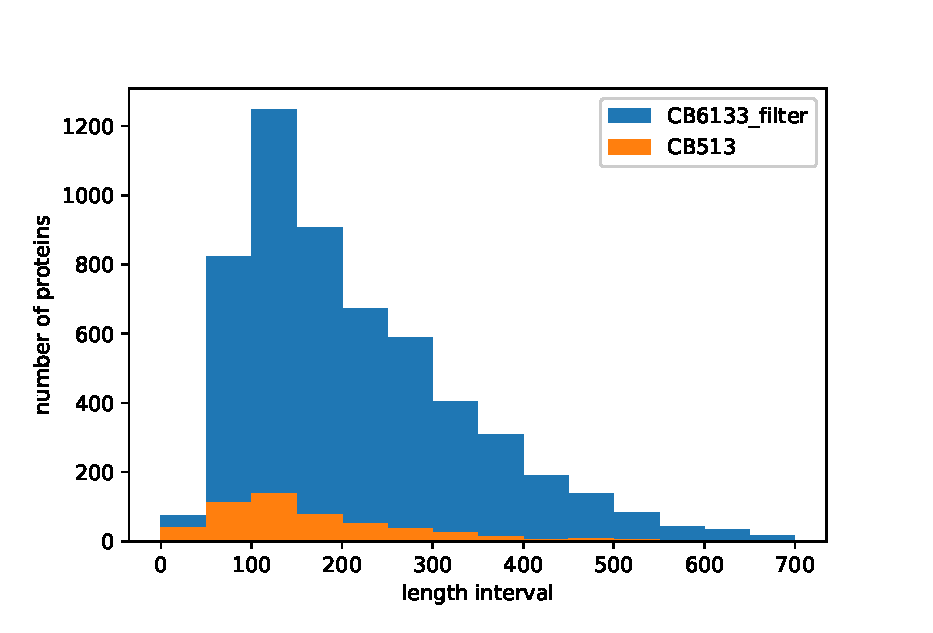
\includegraphics[width=0.7\textwidth]{pic/data_hist}
	\caption{过滤CB6133和CB513中序列长度分布图}\label{fig:5}
\end{figure}

对于上述的数据集,每个残基有57长度的数据通道。‘[0,22)’通道是氨基酸残基;‘[22,31)’通道是八类二级结构标签;‘[31,33)’通道是N-和C末端;‘[33,35)’通道是相对和绝对溶剂可及性;‘[35,57)’通道是序列谱,通过逻辑函数重新定标PSSM(PSSM通过PSI-BLAST从UniRef90数据库导出,E值阈值为0.001和迭代次数为3次)。

\subsection{实验测试}

具体的,深度学习模型用Keras(\url{https://keras.io/})库实现,该库基于深度学习开源框架TensorFlow(\url{https://www.tensorflow.org/})的高级的API。使用Keras默认设置来初始化网络权重,并用自适应学习率的优化器Adam训练所有层,批量大小为32。整个神经网络都在一台带有32GB内存,NVIDIA GTX 1080 Ti GPU,Intel Core i7-8700k CPU的服务器上训练。同时,使用提前停止来防止模型发生过拟合,训练大约需要半天时间。

图6反应了训练损失和验证损失随迭代次数的变化关系,数据来自过滤CB6133数据集,0.4\%的数据用于验证,其余全做训练。

图7是用过滤CB6133迭代20次进行训练,将每次迭代的模型用CB513测试其Q8准确率。可以观察到,在训练集迭代到第10次,测试集的Q8准确率局部最优为68.24\%。

表2给出了算法在CB513测试集上的混淆矩阵。

表3给出了本文算法与三个算法CNF\citep{wang2010protein} ,SC-GSN\citep{zhou2014deep} 和LSTM large\citep{sonderby2014protein} 在CB513数据集上的Q8预测精度对比。


\newpage
\begin{figure}[htbp]
	\centering
	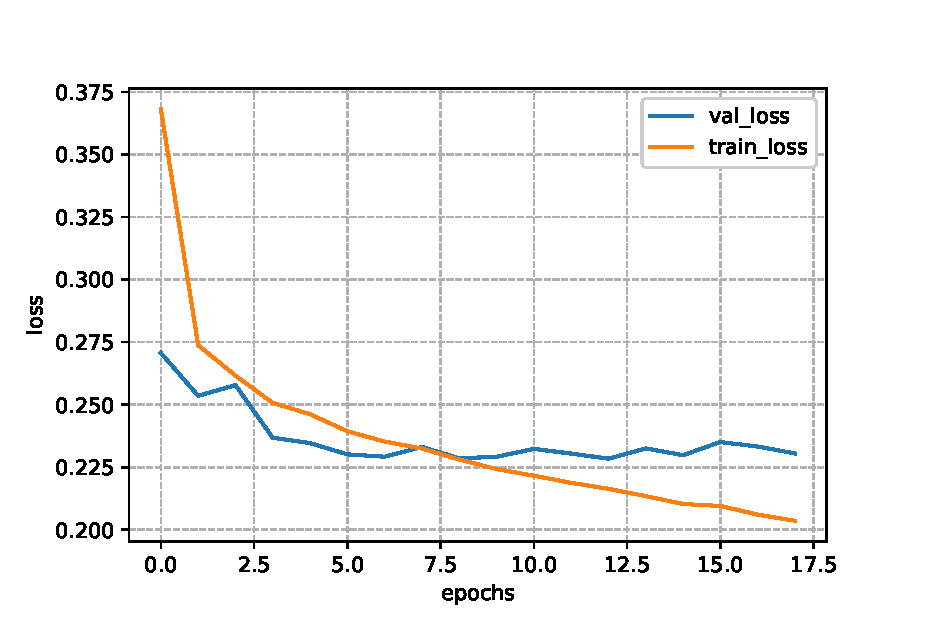
\includegraphics[width=0.7\textwidth]{pic/loss}
\caption{训练损失和验证损失随迭代次数的变化。使用过滤CB6133的99.6\%\\做训练数据,剩余的0.4\%做验证数据。}
\label{fig:fig}
\end{figure}

\begin{figure}[htbp]
	\centering
	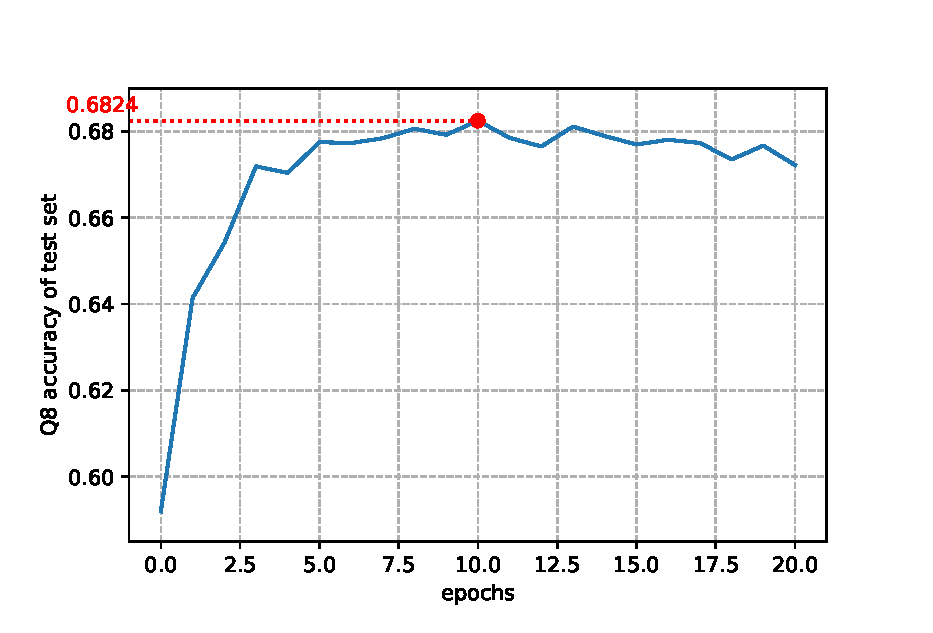
\includegraphics[width=0.7\textwidth]{pic/val_q8}
\caption{CB513\ Q8准确率随训练迭代次数的变化。使用过滤CB6133做训练\\数据,每轮迭代测试一次CB513\ Q8准确率。}
\label{fig:fig}
\end{figure}
\newpage

\begin{table}[htbp]
\renewcommand\arraystretch{1.2}
\caption{算法在CB513测试集上的混淆矩阵}
\center
\begin{tabular}{ccccccccc}
\toprule
 & $H_{pred}$& $B_{pred}$& $E_{pred}$& $G_{pred}$& $I_{pred}$& $T_{pred}$& $S_{pred}$& $L_{pred}$\\
\midrule
$H$& \textbf{92.62}\%& 0.0\%& 0.97\%& 1.1\%&	0.0\%& 2.46\%& 0.3\%& 2.55\%	\\
$B$& 9.14\%& \textbf{1.27}\%& 27.18\%& 0.93\%& 0.0\%& 10.58\%& 5.59\%& 45.3\%\\
$E$& 2.2\%& 0.05\%& \textbf{82.08}\%& 0.46\%& 0.0\%& 2.38\%& 1.53\%& 11.31\%\\
$G$& 27.14\%& 0.0\%& 6.1\%& \textbf{23.63}\%& 0.0\%& 23.21\%& 2.68\%& 17.24\%\\
$I$& 66.67\%& 0.0\%& 3.33\%& 0.0\%& \textbf{0.0}\%& 13.33\%& 3.33\%& 13.33\%\\
$T$& 18.37\%& 0.0\%& 5.38\%& 3.49\%& 0.0\%& \textbf{53.07}\%& 4.49\%& 15.2\%\\
$S$& 8.35\%& 0.02\%& 11.1\%& 1.74\%& 0.0\%& 21.37\%& \textbf{21.38}\%& 36.04\%\\
$L$& 6.17\%& 0.06\%& 17.7\%& 1.03\%& 0.0\%& 8.97\%& 5.48\%& \textbf{60.59}\%\\
\bottomrule
\end{tabular}
\end{table}

\begin{table}[htbp]
\renewcommand\arraystretch{1.2}
\caption{算法在CB513测试集上的分类性能比较}
\center
\begin{tabular}{p{60pt}<{\centering} p{40pt}<{\centering}}
\toprule
算法& $Q_8(\%)$\\
\midrule
CNF& 64.9\%\\
SC-GSN& 66.4\%\\
LSTM large& 67.4\%\\
本文算法& \textbf{68.2}\%\\
\bottomrule
\end{tabular}
\end{table}
\newpage


\section{总结}

本文将深度神经网络应用于蛋白质二级结构预测,融合多种信息:氨基酸残基的类别信息、⽣物的进化信息以及蛋白质序列的组成信息,提出了级联多尺度卷积和双向GRU的端到端模型,用于八类蛋白质二级结构预测。实验结果表明,我们的模型预测效果良好。这种结合局部相邻特征和远程上下文关系的模型架构,可以推广应用到生物信息学领域的其他结构预测问题中。

\newpage
	
\addcontentsline{toc}{section}{参考文献}
\bibliographystyle{abbrv}
\bibliography{bibfile}

\newpage

\begin{center}
\begin{spacing}{1.5}
\bfseries\xiaoerhao\hei Protein Secondary Structure Prediction Base on Cascaded Convolutional and Recurrent Neural Networks
\end{spacing}

\begin{spacing}{1.0}
\xiaosihao\kai College of electronic and information engineering\\
Major:Computer Science and Technology\\
118532014013\qquad Yuan\ Chao\qquad Supervisor: You Wenjie
\end{spacing}
\end{center}

{\bfseries\xiaowuhao\kai 
\subparagraph{\hei【Abstract】}

Protein secondary structure prediction (PSSP) is an important issue in bioinformatics. Inspired by the successes of deep learning in the field of natural language processing (NLP), in this paper, we propose an end-to-end deep neural network model for prediction of eight types protein secondary structure. The model includes four layers: The first layer, the category information of amino acid residues, the evolutionary information of organism and the composition information of protein sequences are encoded and combined, and use the feature embedding to eliminate the sparsity of the 0-1 matrix; The second layer, use the multi-scale convolution to extract the local adjacent features between the amino acid residues; The third layer, use the bidirectional recurrent neural network with GRU to extracts the remote context of protein sequences; The last layer, combine local adjacent features and remote context relationships to predict the secondary structure of eight types. The experimental results show that the deep neural network model proposed in this paper is easy to converge and has good scalability. The model worked well, and achieved 68.2\% $Q_8$ accuracy on the public benchmark CB513.

\subparagraph{\hei【Keywords】}Protein Secondary Structure Prediction; Deep Neural Network
}

\end{document}



































